\documentclass[a4paper,12pt]{article}
\usepackage[a4paper]{geometry}
\usepackage{polski}
\usepackage[polish]{babel}
\usepackage[utf8]{inputenc}
\usepackage{indentfirst}
\usepackage{graphicx}
\usepackage{lastpage}
\usepackage{fancyhdr}
\usepackage{hyperref}
\usepackage{float}
%head & foot
\pagestyle{fancy}
\title{Specyfikacja implementacyjna projektu \textit{Wireworld} w~języku Java}
\author{Chabik Jan (291060), Łuczak Mateusz (291088)}
\date{10 maja 2018}
\setlength\parindent{24pt}
\setlength{\headheight}{16pt}
\lhead{}
\rhead{Specyfikacja implementacyjna projektu \textit{Wireworld} w języku Java}
\rfoot{str. \thepage/\pageref{LastPage}}
\cfoot{}

\begin{document}
\maketitle
\thispagestyle{empty}
\begin{center}
	
\includegraphics[scale=0.1]{logo_ee_big.png}
\end{center}
\newpage

\tableofcontents
\pagenumbering{arabic}
\newpage

\section{Informacje ogólne}
Program jest aplikacją okienkową, w której wszystko obsługiwane jest z poziomu GUI. Okno będzie się pojawiać w centrum ekranu, a jego wielkość wynosić będzie 800x600. Użytkownik będzie miał możliwość wprowadzenia pliku wejściowego do programu w postaci macierzy o wybranej wielkości spośród 25x25, 50x50 i 100x100. Inne będą odrzucone przez program.

Samo GUI będzie zawierać przyciski umożliwiające użytkownikowi wybór pliku wejściowego, katalogu wyjściowego, atrybuty zapisu oraz uruchomienie automatu. Prócz wyżej wymienionych opcji interfejs udostępnia podgląd on-line przejść.

\section{Opis klas i modułów}
Wszystkie klasy znajdują się w pakiecie \texttt{com.wireworld}.
\subsection{Klasa Wireworld}
\begin{itemize}
\item Klasa wykonywalna tworząca GUI i wywołująca metodę obsługującą działanie programu.
\end{itemize}
\subsection{Klasa Matrix}
\begin{itemize}
\item Klasa zawierająca informacje o macierzy;
\item Zawiera metody pozwalające na wypełnienie macierz obwodami i strukturami logicznymi.
\end{itemize}
\subsection{Klasa Simulator}
\begin{itemize}
\item Klasa abstrakcyjna z metodami statycznymi pozwalającymi symulować pojedyncze przejścia automatu \textit{Wireworld}.
\end{itemize}
\subsection{Klasa IOManager}
\begin{itemize}
\item Klasa abstrakcyjna z metodami statycznymi pozwalającymi na sprawdzenie poprawności danych wejściowych, wczytanie ich do programu oraz utworzenie pliku \texttt{.txt} i \texttt{.png}.
\end{itemize}
\subsection{Klasa Options}
\begin{itemize}
\item Klasa typu \textit{singleton} zawierająca informacje o opcjach podanych przez użytkownika;
\item Dostępnymi opcjami są:
	\begin{itemize}
	\item sąsiedztwo (Moore/von Neumann),
	\item ścieżka pliku wejściowego,
	\item ścieżka katalogu wyjściowego,
	\item preferencje dotyczące zapisu (\texttt{.txt} i/lub \texttt{.png}),
	\item informacja o interwale między przejściami automatu.
	\end{itemize}
\item Każda z opcji posiada swój \textit{getter} i \textit{setter};
\item Konstruktor jest prywatny i wywoływany podczas pierwszego odwołania się do metody zwracającej jedyną instancję klasy.
\end{itemize}
\subsection{Klasa GUI}
\begin{itemize}
\item Funkcje GUI są następujące:
	\begin{itemize}
	\item wygenerowanie interfejsu użytkownika,
	\item zapisywanie wprowadzonych przez użytkownika opcji do obiektu \texttt{op\-tions},
	\item umożliwienie użytkownikowi uruchomienie automatu i zarządzanie jego przejściami.
	\end{itemize} 
\end{itemize}
\subsection{Klasa WireStructure}
\begin{itemize}
\item Klasa zawierająca informacje dotyczące wielkości, położenia i orientacji bramek logicznych.
\end{itemize}
\subsection{Klasa Wire}
\begin{itemize}
\item Zawiera informacje o współrzędnych przewodnika.
\end{itemize}
\subsection{Klasy odpowiadające za bramki logiczne (AND, OR, XOR, Diode)}
\begin{itemize}
\item Klasa dziedzicząca po klasie \textit{WireStructure} i stosująca polimorfizm.
\end{itemize}

\section{Metodyka wersjonowania}
\begin{itemize}
\item Wersjonowanie oprogramowania następuje w systemie kontroli wersji Git;
\item Wersje dokumentów obarczone będą nazwą z dopiskiem \texttt{beta} lub \texttt{FINAL}, oraz numerem wersji:
	\begin{itemize}
	\item \texttt{beta} - robocza wersja dokumentu;
	\item \texttt{FINAL} - ostateczna wersja dokumentu;
	\item numer wersji - numer oznaczający aktualną kompilację. Określony zostaje w formacie X.Y, gdzie X to numer kompilacji, a Y numer poprawki. Y jest opcjonalne i występuje tylko przy małych zmianach w~dokumencie (takich jak przykładowo poprawa literówki).
	\end{itemize}
\item Wersje oprogramowania obarczone będą numerem wersji i dodatkową nazwą oznaczającą ważniejsze zmiany (przykładowo GUI v0.2)
\end{itemize}

\section{Kompilator i wersja języka}
Przy tworzeniu naszego oprogramowania używać będziemy języka Java w wersji 8 z kompilatorem \texttt{javac}. Zdecydowaliśmy się na tą wersję z powodu wygody użytkowania oraz dodatkowych opcji, które nie są dostępne we wcześniejszych wersjach (takich jak przykładowo wyrażenia \texttt{lambda}).

\section{Użyte biblioteki}
W naszym programie korzystamy z biblioteki Swing ze względu na łatwość obsługi, dodawania i modyfikacji działania wybranych komponentów, które zostaną użyte w GUI oprogramowania. Prócz Swinga korzystać będziemy ze standardowych bibliotek Javy dostarczanych wraz z \textit{Java Delepoment Kit 1.8}.

\section{Testowanie i konwencja}
Testować działanie programu będziemy za pomocą narzędzi dostępnych w~Frameworku JUnit 4. Dla każdej klasy stworzona zostanie klasa testująca, w której testować będziemy każdą z metod. Skorzystamy z metodyki testów regresywnych, czyli po dodaniu nowej funkcjonalności testować będziemy również poprzednio sprawdzone klasy w celu upewnienia się, czy program działa poprawnie.

\section{Diagram klas}
\subsection{Diagram}
\begin{center}
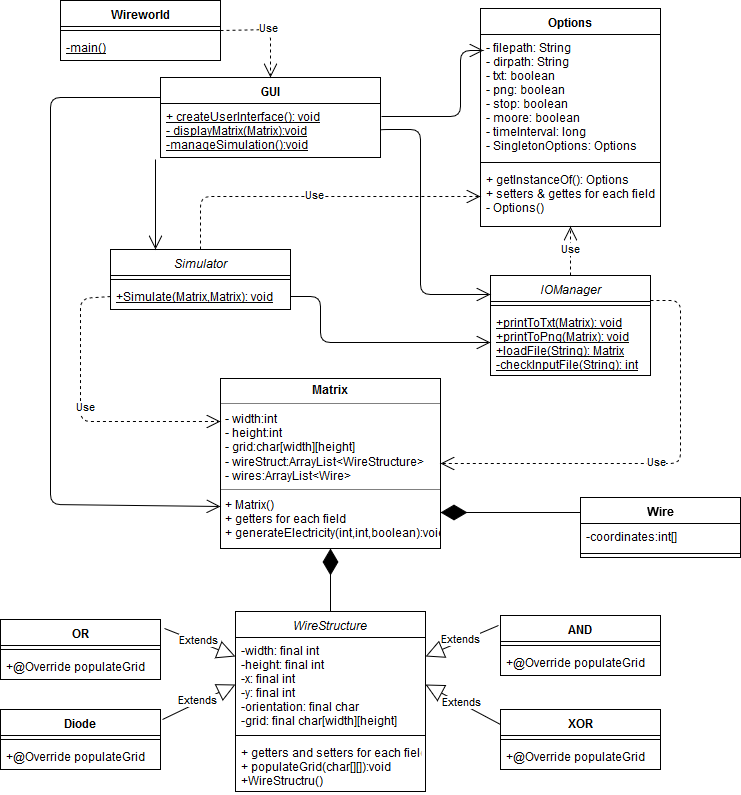
\includegraphics[scale=0.5]{diag.png}
\end{center}
\subsection{Legenda}
\begin{itemize}
\item \underline{Podkreślenie} - Pola i metody statyczne
\item \textit{Kursywa} - Klasa abstrakcyjna
\end{itemize}
\end{document}
